%************************************************
\chapter{Introduction}\label{ch:introduction}
%************************************************

CERN, European Organization for Nuclear Research, (French: Conseil européen
pour la recherche nucléaire) is an European research organization that operates
the largest particle physics laboratory in the world.

Its mission is to: 
\begin{itemize}
	\item Provide a unique range of particle accelerator facilities that enable research at the forefront of human knowledge
	\item Perform world-class research in fundamental physics
	\item Unite people from all over the world to push the frontiers of sciences and technology, for the benefits of all.
\end{itemize}

It host the instrument of the 4 biggest physic collaboration: 
\begin{itemize}
\item ALICE
\item ATLAS
\item CMS
\item LHCb
\end{itemize}

CERN host also a plethora of smaller physical collaborations that benefits from
the instruments, know how, network effect and services availables.

Between the services offered to its users the computing service is one of the
most interesting. Indeed CERN host and manage one of the biggest computing
data center used for public research.

An issues that affect the operations inside the data center is the provisioning
of software on the computing servers.

A specialization of the same problem is the provisioning of containers images.

The general problem of software provisioning is been solved by the use of
CernVM-FileSystem \cite{cvmfs}, a read only file-system that provides a scalable, reliable
and low maintenance software distribution system.

This thesis will explore the problem of creating a suitable read-only
file-system structure to provision containers images on computing nodes. We
will provide a general read-only file-system structure and we will implement the
proposed methodology on top of CVMFS.

This thesis is composed by several parts: The background will provide the
necessary information on the CERN computing architecture (WLCG), then we will
explore CVMFS and why it is a good fit for the CERN computing architecture, the
last part of the background will cover the integration between CVMFS and
containers technologies.  The state of the art will explore what alternatives
are available for software distribution in general and for distribution of
images.  We will then define the problem that this thesis is trying to solve
and few metrics of interest in our specific case.  The methodology part will
explain the details of the solution we propose for this specific problem.  The
implementation chapter will focus on how the proposed methodology is been put
in practise.  We will evaluate the result of the proposed methodology and
implementation on the result part following the metrics that were previously
proposed.  Finally we will propose future work and enhancement to the
implementation

\chapter{Background}\label{ch:background}

In this chapter we are going to introduce the concept and the technologies that
made this work possible.  We will start introducing the Worldwide LHC Computing
Grid (WLCG), which is the \textit{collaboration} that provide the computing power
necessary to the CERN mission. The dimension of the WLCG and its specific
workload required and allowed a specific software distribution system,
CernVM-FileSystem which is used to provision the machines on the WLCG.

Then we will introduce the concept of containers, a different way to solve the
software distribution problem that is widely adopted in the industry. In
particular, we will focus on Docker containers and the Docker images format. We
will then explore Singularity, a container runtime capable of running
containers images stored as simple folder in the filesystem. Finally we will
explore the Docker \texttt{cvmfs/graphdriver}, a Docker plugin that allow to
run Docker images whose content is available on a read-only file-system without
the need of downloading or accessing the Docker standard images.


\section{WLCG}

The Worldwide LHC Computing Grid is an global collaboration of more than 170
data centers in 42 countries.  The mission of the WLCG is to provide the
computing resources to store, distribute and analyze the data generated by the
operations of the LHC \cite{grid:website},\cite{grid:report}.

The organization of the WLCG follows a hierarchical model, where each level of
the hierarchy is called “Tier”. The most central Tier is the Tier-0, which is
hosted by CERN in the Geneva Area and in Budapest. There are 13 Tier-1 data
centers with enough storage and computing capabilities to support the Grids
operation around the clock.
Tiers-1 are geographically distributed: 8 of them are in
Europe, 3 in North America and the rest is in Asia. Finally, the Tier-2 data
centers do not have strict requirements and are generally operated by research
centers and universities \cite{grid:report}.  A schematic representation of the
architecture of the WLCG is provided on Figure \ref{fig:wlcg-schema}.


\begin{figure}
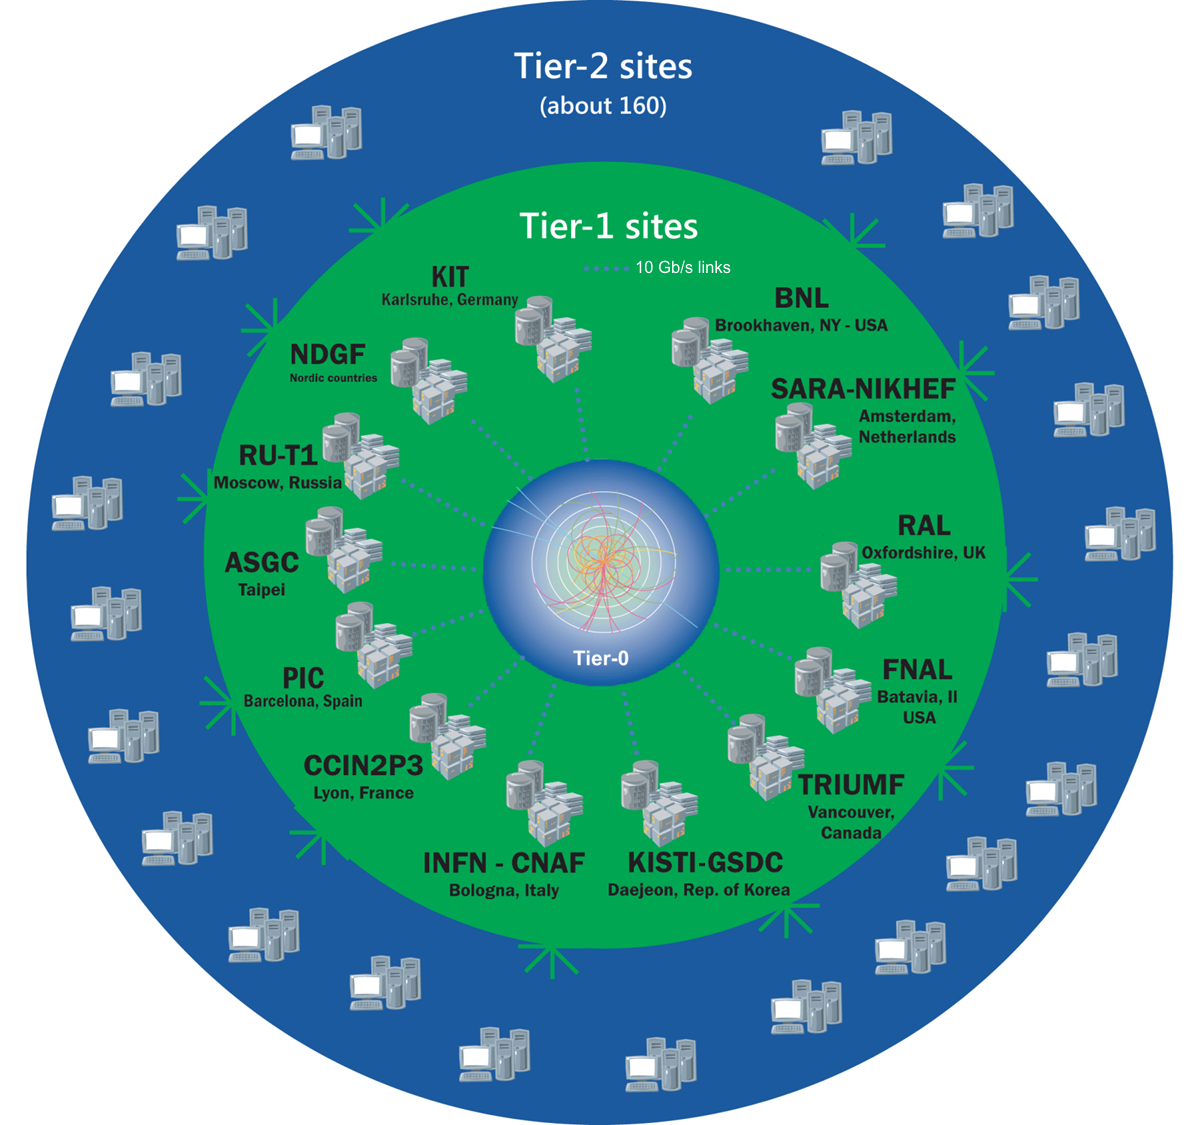
\includegraphics[width=\textwidth,height=\textheight,keepaspectratio]{gfx/WLCG}
\caption{Schematic representation of the WLCG}
\label{fig:wlcg-schema}
\end{figure}

The work of the WLCG is mostly divided in two big classes: analysis of the data
from the LHC detectors and Monte Carlo simulations.  The WLCG assume and
support a batch computing paradigm. Analysis and simulations are split in
smaller jobs that are distributed to different computing node that can work in
parallel \cite{grid:report}, \cite{grid:update}.

Before to start each job it is necessary to install the software on the server.
Unfortunately the amount of software potentially needed in each computing node
and the velocity at which the software is updated can make the installation
challenging. Moreover, simpler installation techniques that rely on packages
managers are not applicable since they would put the centralized package
managers themselves under too much load. Several solution have been proposed
and used in the past, eventually it settled for the use of CernVM-FileSystem
(CVMFS) \cite{cvmfs}.

\section{CVMFS}

This section will explore CernVM-FileSystem, we will start with an high level
overview of CVMFS, then we will explore what happens when a file is requested.

% need to really talk about the sub-catalog system

\subsection{CVMFS High Level Overview}

CernVM-FileSystem \cite{cvmfs} provides a scalable, reliable and
low-maintenance software distribution system. It is implemented as a read-only
POSIX file-system in user space exploiting FUSE (File-system in USErspace)
\cite{fuse} and standard web server technologies such as Apache or NGNIX.

Each running instance of CVMFS provides a read-only file-system that is
denominated \textit{repository}. At CERN different collaborations maintains
different repositories, but all of them can be mounted from all the computing
node in the WLCG. CVMFS is engineered to support repository of size on the
order of the Terabyte with billions of files.

To save storage space files are addressed by their content (Content Addressable
Storage), hence duplicated files will be stored only once.

In order to distribute software to geographically distant data centers and keep
a low latency, CVMFS allows to cache content in different machines. This allow
to host a cache server in each Tier of the WLCG. The use of caches fits
perfectly with the Tiers models of the WLCG presented above. The Tier-0 host
the main repository (Stratum-0), and the Tier-1 host the first level of cache
(Stratum-1) and so on.

The content of the files are served using the HTTP protocol by a standard
web server. The files are lazily downloaded only on the machine that need them
and only when necessary.

In order to locate and request files from CVMFS the clients download the
catalog, a simple SQLite database which describes a subtree of the whole
file-system.  The catalog contains all the metadata of files and directories,
including owner, group, permission, and size. Moreover the catalog contains
also the URL where to download the files.

A root catalog is available in a know path, and, if the file-system grows too
large, the root catalog links to other sub-catalogs. The use of sub-catalogs
allows to keep each catalog small improving the query time.

\subsection{CVMFS Details}\label{subsec:cvmfs-details}

CVMFS is implemented using the Client-Server architecture. The server is
responsible to manage the content of the repository and to expose it via HTTP
API.  The client is installed in the host machine and is responsible to expose
the content of the repository to the users and it is implemented as a FUSE
daemon which implements all the system calls necessary for a read-only
file-system.

When a CVMFS file-system is mounted, it starts by reading a configuration file
which describes each repository. The client then downloads a simple text file
which points to the catalog of the repository. Once the catalog is downloaded
the client has all the information necessary to start responding to the system
calls performed by the user.

As an example, when the user requires a \texttt{stat} system call against a
file, the client reads from the catalog all the information about the file
like, size, permission, mode, etc.. and replies with them. Instead when the
user requires to read from a file, the client first downloads the file from the
server, stores it into a local cache and passes through each read operation to
the local copy.

This approach allows to download only the file really required, since all the
other system calls can be served by just reading from the catalog. However this
implies that the reading latency from a file depends on the network latency.
This strategy works very well if the reading latency of a file is not a major
concern and if reading from the catalog is fast. However, if the catalog grows
too big, then the queries become too slow. 

To overcome this limitation the sub-catalogs were introduced.  A sub-catalog is
exactly like the normal catalog, but while the catalog refers to the whole
file-system tree, a sub-catalog refer to a smaller sub tree of the file-system.
In order to avoid confusion, we will refer to the root-catalog as the catalog
that includes the root of the file-system and to sub-catalog to all the other
catalogs in the file-system. The root-catalog, of course, embeds several
sub-catalogs, and each sub-catalog can, recursively, embed another sub-catalog.

When is required to read information about a file, the client starts by looking
into the root catalog and then it follows the sub-catalogs structure until it
finds the required file.

\section{Containers}
\label{sec:containers}

While CERN solved its problems of software distribution with CVMFS the industry
opted for a different approach: containers. 
Containers are a standard units of software that package up code and all its
dependencies so that computer applications run quickly and reliably from one
computing environment to another \cite{docker:what}.1

In order to standardize containers and make the technology interoperable in
2015 the \textit{Open Container Initiative (OCI)} was founded \cite{oci}. The
OCI defined a standard format to use to pack containers into \textit{images}
\cite{oci-image-spec}, this format have been adopted by Docker and that is used
in the \textit{Docker Images}.
A Docker image is an immutable
set of tar files, where each tar file is called layer. Prior to run the container,
each layer gets mounted one on top of the other to re-create the original
environment where to run the application \cite{oci:image-filesystem}. The
content of each image is codified in a \texttt{json} file, the manifest, which
provides the unique name of the image itself and which refers to each layer that
compose the image by their unique identifiers. The unique identifier of both
images and layers is the result of the function \texttt{hash256} of their
content \cite{oci:content}. 

Docker images are distributed through Docker registries, simple HTTP servers
that given the unique identifiers of a layer provide the layer itself,
similarly, given the identifier of an image the registries provides its
manifest \cite{docker:registry}.

Docker allow to associate a human readable identifier to each image, this name
is composed by a namespace, which identifies the user or organization that created
the image, a name, which identifies the image itself and a tag, which identifies
the version of the image. These names are not immutable and are meant to be
used just by humans to recognize and use the images \cite{docker:tag}.
The repository where the image is hosted, its namespace, its name and its tag
create a hierarchical structure between the several images that is easy to
navigate for humans.

\subsection{Docker and the cvmfs/graphdriver plugin}
\label{subsec:docker-thin-images}

Docker is a thin CLI layer on top of a Linux daemon, \texttt{dockerd} which is
responsible to obtain the Docker images from the registries, mount the layers,
manage the runtime of the image and allow communication of a Docker runtime
with the host system \cite{docker:overview}.

Docker layers can be shared between different images, so the Docker daemon
download them once and store them in the local machine for future use
\cite{docker:storage}. On average less than 7\% of the content inside a Docker
image is used during the runtime of the image \cite{slacker}. The layers are
distributed as a single tar file \cite{oci:image-filesystem}, hence a naive
distribution of layers with CVMFS would not provide any advantage. The whole
tar files would need to be downloaded erasing the advantages of using CVMFS.

A solution to this problem was introduced with the \texttt{cvmfs/graphdriver}
plugin and the concept of "thin-images" \cite{graphdriver-plugin}. In this work
we are not interested in the internal of the \texttt{cvmfs/graphdriver} plugin,
it will be sufficient to know that the Docker daemon can be enhance with the
use of plugins \cite{docker:plugin} and that the plugin allows us to run what
are called "thin-images".

\textit{Thin-images} are Docker images that are created starting from standar
(\textit{fat}) Docker images. The content of a \textit{thin-image} is only a
simple \texttt{json} file whose content is the list of layers needed by the
original \textit{fat-image} and where to find them in the host file-system, we
call this file the \textit{recipe} an example of \textit{recipe} file is show
on Listing \ref{lst:thin-example}. \textit{Thin-images} can be executed only if
the Docker daemon have enabled the \texttt{cvmfs/graphdriver} plugin, indeed
the plugin is able to read the content of the thin-image, mount the original
layers inside the container, and finally execute the application
\cite{graphdriver-plugin}.

\begin{minipage}{\linewidth}
\begin{lstlisting}[caption={Example of a \textit{recipe} file of a Docker \textit{thin image}},label={lst:thin-example}]
{
  "version": "1.0",
  "origin": "https://registry.hub.docker.com/library/python:latest",
  "layers": [
    {
      "digest": "bc9ab7...0257b7",
      "url": "cvmfs://thin.osg.cern.ch/.layers/bc/bc9ab7...0257b7/layerfs"
    },
    {
      "digest": "193a63...110d7f",
      "url": "cvmfs://thin.osg.cern.ch/.layers/19/193a63...110d7f/layerfs"
    },
    {
      "digest": "e5c3f8...818580",
      "url": "cvmfs://thin.osg.cern.ch/.layers/e5/e5c3f8...818580/layerfs"
    },
    {
      "digest": "b61a0d...b615a9",
      "url": "cvmfs://thin.osg.cern.ch/.layers/b6/b61a0d...b615a9/layerfs"
    }
  ]
}
\end{lstlisting}
\end{minipage}



If the files necessary to run the \textit{thin-images} are distributed by CVMFS, it is
possible to run docker containers without downloading any unnecessary content.

Moreover the \texttt{cvmfs/graphdriver} plugin is able to run standard (\textit{fat})
Docker images, hence conventional Docker images are supported seamlessly \cite{graphdriver-plugin}.

On figure \ref{fig:flowchart-run-thin-image} we show how the plugin decides how
to mount the container file system. If it detects that the image is a standard
\textit{fat} Docker image it run it as a standard image, if it detect that is a
\textit{thin} image it mounts the layers from the CVMFS read-only file system.

\begin{figure}
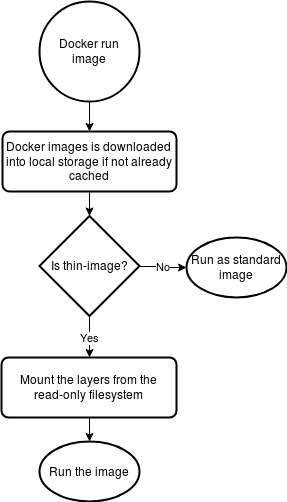
\includegraphics{gfx/RunThinImages}
\caption{Decision proces for running docker thin images}
\label{fig:flowchart-run-thin-image}
\end{figure}

The downside of this approach is that a "thin-image" can be downloaded, store in
the local storage and successfully run using the content provide by CVMFS. On a
second moment the images can be update, uploaded newly on the registry and the
old content in CVMFS is deleted to host the new content of the image. If now
the user try to run the same images, it will not download it again from the
registry but it will use the image already cached, referring
to content not available anymore on CVMFS, hence it will fail to run.

\subsection{Singularity}

Singularity \citep{singularity:home} is another container runtime, it provides
its own image format but is capable to run standard Docker images
\cite{singularity:docker} as well.  Moreover it is capable of running
containers, also Docker containers, directly from a directory containing the
unpacked container file-system itself \cite{singularity:run}.

Given the Singularity capability to run Docker containers directly from a
directory containing the unpacked Docker image file-system its integration with
CVMFS is simpler that the one with Docker itself. Indeed it is sufficient to
host the directory containing the unpacked file-system of the Docker image in
CVMFS.

\section{Problem Definition}

We have introduce how CERN has overcome the challenges of software distribution
using CVMFS. Unfortunately this is not enough since run-time dependencies
between software components can break application that instead are running
perfectly fine in a different environment.

Since containers pack up all their runtime dependencies in a standard
environment they are a suitable solution for this problem. However containers
are distributed as big tar files which is against the design and working
principle of CVMFS.

Both CVMFS and containers aims to solve the similar problem of server
provisioning, however they made different trade-offs. CVMFS opted for an
efficient distribution of the content, however this makes difficult and
inconvenient to pack all the runtime dependencies of a particular application.
Containers opted to make each application self-contained so that the
application can run reliably also on different computer environment, however
they loose efficiency in the distribution of their content.

We don't believe that efficient content distribution and application
containerization are contrasting goals, hence in this thesis will attack the
problem of how to efficiently distribute the content of containers.

In Chapter \ref{ch:Methodology} we will present a generic read-only file system
structure suitable to host container content.  In Chapter
\ref{ch:Implementation} we will show how we implemented such read-only file
system structure on CVMFS in order to distribute containers content. Finally we
will show the result of such work on Chapter \ref{ch:Results}. Possible
enhancement to this work are finally exposed on Chapter \ref{ch:FutureWorks}.

